% =====================================================================
% ACS Omega resubmission (ao-2026-09173w) -- REBUILT AROUND THE N3 BENCHMARK, draft 2026-11-17
%
% ACS `achemso` class (manuscript=article). Bibliography style is owned by achemso -- do NOT add
% \bibliographystyle or load natbib. ACS Omega places Methods AFTER Conclusions.
%
% EVERY N3 NUMBER comes from generated/*.tex, written by scripts/n3_paper_numbers.py from
% results/n3/n3_results.json (committed f1c713a, before interpretation). Never type a result by hand.
% CLAIM RULES: tasks/n3_protocol.md section 4 (outcome -> claim map), section 5 (frozen Table R
% wording) and section 6 (abstract rules). Forbidden: any CSP/end-to-end claim for OURS; "better than
% physics-based search"; any representability claim against MolCrystalFlow's per-copy representation.
% The pre-N3 version is archived in archive/main-archive-2026-11-17-pre-N3.tex.
% =====================================================================
\documentclass[journal=acsodf,manuscript=article]{achemso}

\usepackage{amsmath,amssymb}
\usepackage{graphicx}
\usepackage{booktabs}
\usepackage{xcolor}
\usepackage{rotating}
\graphicspath{{figures/}{../../figures/}}

% GENERATED by scripts/n3_paper_numbers.py from results/n3/n3_results.json -- do not edit
\newcommand{\nN}{1{,}000}
\newcommand{\nOursPick}{8.47}
\newcommand{\nOursSd}{1.35}
\newcommand{\nOursSeeds}{8.5, 7.1, 9.8}
\newcommand{\nOursDraw}{0.98}
\newcommand{\nOursAny}{13.6}
\newcommand{\nOursSec}{16.8}
\newcommand{\nOursNtwoPick}{6.47}
\newcommand{\nOursNtwoSd}{0.32}
\newcommand{\nSearchPick}{99.4}
\newcommand{\nIEPick}{58.9}
\newcommand{\nMcfRPick}{0.00}
\newcommand{\nMcfRGPick}{0.13}
\newcommand{\nIvPPick}{0.00}
\newcommand{\nIiSPick}{0.97}
\newcommand{\nFloorPick}{0.01}
\newcommand{\nHaarPick}{0.17}
\newcommand{\nPressPick}{0.17}
\newcommand{\nIvSPick}{0.20}
\newcommand{\nMcfAPick}{0.00}
\newcommand{\nHOneDelta}{+8.33}
\newcommand{\nHOneCI}{[7.30, 9.40]}
\newcommand{\nHOneP}{$5.9\times10^{-61}$}
\newcommand{\nHTwoDelta}{$-$90.93}
\newcommand{\nHTwoCI}{[$-$92.00, $-$89.70]}
\newcommand{\nHTwoP}{$1.4\times10^{-298}$}
\newcommand{\nHThreeDelta}{+8.47}
\newcommand{\nHThreeCI}{[7.47, 9.53]}
\newcommand{\nHThreeP}{$3.0\times10^{-67}$}
\newcommand{\nHOneNtwoDelta}{+6.33}
\newcommand{\nHOneNtwoCI}{[5.47, 7.33]}
\newcommand{\nHOneNtwoP}{$9.5\times10^{-46}$}
\newcommand{\nHTwoNtwoDelta}{$-$92.93}
\newcommand{\nHTwoNtwoCI}{[$-$93.90, $-$91.83]}
\newcommand{\nHTwoNtwoP}{$7.2\times10^{-299}$}
\newcommand{\nHThreeNtwoDelta}{+6.47}
\newcommand{\nHThreeNtwoCI}{[5.60, 7.43]}
\newcommand{\nHThreeNtwoP}{$1.3\times10^{-51}$}
\newcommand{\nHOneRDelta}{+8.47}
\newcommand{\nHOneRCI}{[7.47, 9.53]}
\newcommand{\nHOneRTwo}{[6.70, 10.30]}
\newcommand{\nHOneGDelta}{+8.33}
\newcommand{\nHOneGCI}{[7.30, 9.40]}
\newcommand{\nHOneGTwo}{[6.57, 10.20]}
\newcommand{\nHOneTwo}{[6.57, 10.20]}
\newcommand{\nHTwoTwo}{[$-$92.80, $-$88.97]}
\newcommand{\nHThreeTwo}{[6.70, 10.30]}
\newcommand{\nLearnDelta}{+7.50}
\newcommand{\nLearnCI}{[6.47, 8.65]}
\newcommand{\nExpDelta}{+0.83}
\newcommand{\nExpCI}{[0.53, 1.20]}
\newcommand{\nZmcfMin}{+8.18}
\newcommand{\nFloorDelta}{+8.45}
\newcommand{\nFloorCI}{[7.45, 9.53]}
\newcommand{\nIEvsSearchDelta}{$-$40.50}
\newcommand{\nIEvsSearchCI}{[$-$42.53, $-$38.40]}
\newcommand{\nFFAnchN}{983}
\newcommand{\nFFDriftN}{2}
\newcommand{\nFFUnresN}{15}
\newcommand{\nAnchDelta}{$-$91.08}
\newcommand{\nAnchCI}{[$-$92.17, $-$89.93]}
\newcommand{\nAnchPct}{98.3}
\newcommand{\nOmcN}{818}
\newcommand{\nOmcDelta}{$-$90.26}
\newcommand{\nOmcCI}{[$-$91.52, $-$88.92]}
\newcommand{\nOursGeoMed}{129}
\newcommand{\nOursEns}{12.4}
\newcommand{\nRLegacy}{649}
\newcommand{\nRLegacyCentro}{604}
\newcommand{\nRMixed}{634}
\newcommand{\nRMixedMiss}{634}
\newcommand{\nRMixedApprox}{323}
\newcommand{\nOursStratMin}{4.58}
\newcommand{\nOursStratMax}{9.52}
\newcommand{\nSearchStratMin}{97.3}
\newcommand{\nSearchStratMax}{100.0}

\makeatletter
\newcommand{\inputrows}[1]{\@@input #1 }
\makeatother
\newcounter{todocount}
\DeclareRobustCommand{\TODO}[1]{\stepcounter{todocount}\textcolor{red}{[TODO: #1]}}
\DeclareRobustCommand{\CITEME}[1]{\stepcounter{todocount}\textcolor{red}{[CITE: #1]}}
\AtEndDocument{\typeout{[symmc-flow] TODO/CITE markers remaining: \thetodocount}}

\author{Frank Cai}
\affiliation{Purdue University, West Lafayette, Indiana 47907, United States}
\email{cai485@pfw.edu}

% Title: provisional (Frank to confirm). The protocol rules out "structure prediction" (P section 0).
\title{Exact Space-Group Expansion of a Learned Asymmetric Unit: A Preregistered
Benchmark of Molecular-Crystal Orientation Completion}

\keywords{molecular crystals, space-group symmetry, orientation, flow matching,
preregistration, benchmark}

\begin{document}

\begin{tocentry}
\centering
\TODO{new TOC graphic; the old one shows the superseded method}
\end{tocentry}

\begin{abstract}
\noindent
Rigid-body generative models of molecular crystals predict an orientation for every
molecule in the cell, although space-group symmetry fixes all of them once the
orientation of the asymmetric unit is known. We test, in a preregistered benchmark,
a flow model that predicts only the asymmetric-unit orientation and builds the crystal
by exact space-group expansion. The task is orientation completion, not crystal
structure prediction: for a crystal with one molecule in the asymmetric unit, the true
lattice, space-group operations, asymmetric-unit centroid and rigid conformer are given,
and the asymmetric-unit orientation is predicted. On \nN{} held-out crystals from the
Cambridge Structural Database, scored once under a frozen protocol, the model reproduces
the experimental structure for \nOursPick{}~$\pm$~\nOursSd\% of crystals (one selected
structure per crystal; mean $\pm$ s.d.\ over three trained models). Three hypotheses
were tested with Holm correction. Against MolCrystalFlow retrained on the same data and
given the true lattice and the true centroids of every molecule (H1), the difference is
\nHOneDelta{} percentage points (pp; BCa 95\% CI \nHOneCI), and H1 is supported. Against
a search over the asymmetric-unit orientation with a universal interatomic potential,
given the same information (H2), the difference is \nHTwoDelta{} pp \nHTwoCI: H2 is not
supported, because the search reproduces \nSearchPick\% of the structures. Against our
previous architecture (H3), the difference is \nHThreeDelta{} pp \nHThreeCI, and H3 is
supported. Among the learned models tested, predicting the asymmetric unit and expanding
it exactly did better on this task; with this much information given, physics-based
search remained far more accurate.
\end{abstract}

% =====================================================================
\section{Introduction}
% =====================================================================
Crystal structure prediction (CSP) seeks the stable periodic packing of a chemical
system, and generative models have become a fast alternative to large ensembles of
energy evaluations, progressing from crystal diffusion autoencoders\cite{xie2022cdvae}
to joint equivariant diffusion\cite{jiao2023diffcsp} and Riemannian flow
matching\cite{miller2024flowmm,lipman2023flowmatching,chen2024riemannian}. Rigid-body
factorization suits molecular crystals: freezing each molecule's conformer reduces
dozens of atomic coordinates to a lattice, a fractional centroid and an orientation in
$\mathrm{SO}(3)$ for every molecule.

Space-group symmetry makes most of those orientations redundant. In a crystal with one
molecule in the asymmetric unit ($Z'=1$) on a general position, the $K$ molecules of the
cell are the images of a single molecule under the $K$ operations $(W_k, w_k)$ of the
space group: each copy's centroid and atoms follow from the asymmetric-unit molecule by
the operation, and an improper operation ($\det W_k=-1$) also mirrors the conformer. One
orientation, that of the asymmetric unit, $R_{\text{asym}}$, therefore fixes all $K$.
Current rigid-body molecular-crystal generators do not use this.
MolCrystalFlow\cite{zeng2026molcrystalflow} generates an orientation for every molecule
and imposes no space-group constraint, and MOFFlow\cite{kim2025mofflow} generates the poses
of rigid building blocks of metal--organic frameworks. Space-group symmetry has been built into
generators of inorganic crystals, through Wyckoff positions or space-group-constrained
coordinates\cite{jiao2024diffcsppp,wyckoffdiff2025,symmcd2025,puny2025sgfm,mu2026nextcrystal};
none of these generates rigid molecules. For molecular crystals, SALA\cite{cai2026sala}
generates conformation, lattice and packing end to end from a molecular graph and a space
group by evolving asymmetric-unit atomic coordinates; the present benchmark addresses a
narrower task, completing the orientation of a rigid asymmetric unit when the lattice,
operations and position are given.

We ask whether this redundancy matters for learned models, in a benchmark that compares
enforced symmetry together with our learner against learned independent-copy models and
classical searches. Every arm receives
specified information about each crystal (Table~\ref{tab:info}), every learned comparator
is retrained on the same training set with its released code, and every arm is scored
once, on \nN{} held-out crystals from the Cambridge Structural Database
(CSD)\cite{groom2016csd}, by one scoring script under hypotheses, statistics and claim
rules fixed in advance. The task is \emph{orientation completion}: given the true
lattice, the true space-group operations, the true asymmetric-unit centroid and the rigid
conformer of a $Z'=1$ crystal, predict $R_{\text{asym}}$. This is not crystal structure
prediction. The lattice, space group, $Z$, $Z'$ and molecular position are oracle inputs,
and no claim in this paper extends beyond that task.

The benchmark gives three results.
\begin{itemize}\itemsep0.05em
\item \textbf{Representability.} Exact expansion with the full operations, proper and
improper, represents every test crystal, whereas the proper-rotation pipeline of our
previous architecture cannot represent \nRLegacy{} of the \nN{} (Table~\ref{tab:repr}).
\item \textbf{Against learned comparators.} A flow model that learns $R_{\text{asym}}$ and
expands it exactly reproduces \nOursPick~$\pm$~\nOursSd\% of the test structures.
MolCrystalFlow, retrained on our training set and given the true lattice and the true
centroids of all copies, and our previous architecture reproduce almost none, and both
preregistered comparisons (H1, H3) are supported.
\item \textbf{Against physics-based search.} A search over $R_{\text{asym}}$ with a
universal interatomic potential, given the same information, reproduces \nSearchPick\%
of the structures. The preregistered comparison (H2) is not supported, and we report it
as such.
\end{itemize}

% =====================================================================
\section{Definitions and a Worked Example}
% =====================================================================
Throughout, a crystal has one molecule in its asymmetric unit ($Z'=1$) on a general
position, so its unit cell holds $Z=K$ molecules, where $K$ is the number of operations of
the space group in the crystal's own setting. We use the following terms.
\begin{description}\itemsep0.1em
\item[Operation.] A space-group operation $(W_k,t_k)$ maps fractional coordinates
$c\mapsto W_kc+t_k$. It is \emph{proper} if $\det W_k=+1$ (a rotation or screw axis) and
\emph{improper} if $\det W_k=-1$ (an inversion, mirror or glide).
\item[Asymmetric-unit molecule and copies.] The asymmetric-unit molecule is one molecule
of the cell, with fractional centroid $c_0$ and a rigid conformer (its atom positions
about the centroid, held at the experimental geometry). The $K$ molecules of the cell are
its \emph{copies}: copy $k$ is the image of the asymmetric-unit molecule under operation
$k$, and copy 1 (the identity) is the asymmetric-unit molecule itself.
\item[Orientation and $R_{\text{asym}}$.] An orientation is a rotation in $\mathrm{SO}(3)$
that places the conformer in the cell; $R_{\text{asym}}$ is the orientation of the
asymmetric-unit molecule.
\item[Handedness.] An improper operation turns the conformer into its mirror image. For a
chiral conformer this is the opposite enantiomer, so the copy has the opposite handedness to
the asymmetric-unit molecule.
\item[Exact expansion.] Building all $K$ copies from $c_0$, $R_{\text{asym}}$ and the
conformer by applying each operation to the atoms (eq~\ref{eq:expand} in Methods). Because
the operation acts on atoms, an improper operation produces the mirrored copy directly; no
rotation is assigned to it.
\item[Orientation flow.] A generative model that turns random rotations into a predicted
rotation by integrating a learned velocity field on $\mathrm{SO}(3)$. OURS draws
$R_{\text{asym}}$ this way (Methods).
\end{description}

\paragraph{Worked example.} Figure~\ref{fig:worked} shows a training-set crystal in
$P2_1/c$ ($K=4$; CSD refcode LAJKOX, C$_7$H$_{15}$N$_3$O$_2$). Its four operations are the
identity, a twofold screw axis (proper), an inversion centre and a glide plane (both
improper). Given $R_{\text{asym}}$, the identity copy is the asymmetric-unit molecule, the
screw copy is its rotated image, and the inversion and glide copies are its mirror images.
The given centroid and operations fix where each copy sits and which copies are mirrored;
one predicted rotation, three numbers, then fixes all four orientations. A model that predicts an orientation for every copy must learn these
relations from data and needs a separate mirrored conformer for each improper copy; a model
that predicts only $R_{\text{asym}}$ obtains them exactly from the operations.

\begin{figure}
\centering
\IfFileExists{figures/fig_n3_worked_example.pdf}{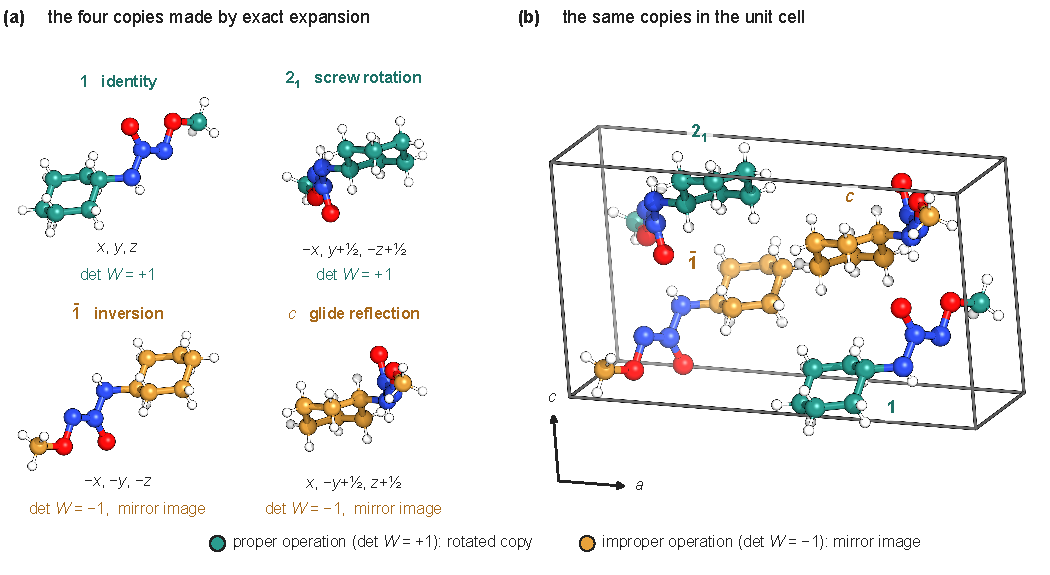
\includegraphics[width=\linewidth,height=0.72\textheight,keepaspectratio]{fig_n3_worked_example}}{\TODO{figure: worked example}}
\caption{Worked example: training crystal LAJKOX ($P2_1/c$). (a) The cell viewed along $b$,
with the copies coloured by the operation that generates each; the hatched copies come from
improper operations ($\det W_k=-1$) and are mirror images. (b) Exact expansion
(eq~\ref{eq:expand}): copy $k$ has centroid $c_k=W_kc_0+t_k$ and atoms placed by
$C_kR_{\text{asym}}$ about it, so one predicted rotation gives every copy. Glyphs show each copy's conformer up to a
proper rotation; H atoms are omitted. Generated by \texttt{scripts/fig\_n3\_worked\_example.py}.}
\label{fig:worked}
\end{figure}

\paragraph{Terms from the earlier version of this work.} Each molecule's conformer is
stored in its own coordinate frame, its \emph{body frame}, and which orientation counts as
the identity is a free choice, the \emph{gauge}. Our earlier manuscript chose one copy as
the \emph{reference copy} and \emph{re-gauged} the crystal, expressing each copy's
orientation $R_k$ relative to the reference as $R_kR_0^{\top}$. It also conditioned the
model on a \emph{coset label} that identified the operation generating each copy. For a
proper operation $R_kR_0^{\top}=C_k$ (eq~\ref{eq:expand}), so that relative orientation is
fixed analytically by the operation and never needed to be learned. For an improper
operation, it is not a rotation of the same conformer. The present design learns only
$R_{\text{asym}}$ and lets the operations supply everything else exactly. The comparison arm
iv-P (H3) is the earlier architecture retrained on this task: it receives per-copy operation
labels and mirrored conformers and predicts every copy's absolute orientation. The earlier
manuscript's relative-target experiment itself was not rerun.

% =====================================================================
\section{Results and Discussion}
% =====================================================================
\subsection{Benchmark design}
\begin{table}[t]
\caption{Information given to each arm. For the MolCrystalFlow (MCF) arms,
``copies'' means $z_{\mathrm{MCF}}$, the number of molecules in the exported MCF
cell: $K$ for primitive lattices and $K/\mathrm{mult}$ for centred ones, where
mult is the centring multiplicity (lattice points per cell). MCF-R is not given the operations, but
spglib on the true centroids, keeping the operations consistent with each copy's
handedness, recovers the copy-to-copy rotations uniquely in 198 of 200 DEV-TEST (development-set)
crystals (the truth is among the candidates in the other 2). H1 therefore tests
explicit, enforced symmetry together with our learner; the ii-S ablation
separates the two.}
\label{tab:info}
\small
\begin{tabular}{@{}p{2.3cm}p{2.9cm}p{2.6cm}p{3.0cm}p{2.5cm}@{}}
\toprule
 & OURS and CLASSICAL & iv-P (old architecture) & MCF-R and MCF-R+G & MCF-A (context) \\
\midrule
lattice & true & true & true (primitive if centred) & generated \\
centroids & $c_0$ true; copies from the operations & all $K$ true & all $z_{\mathrm{MCF}}$ true & generated \\
space-group operations & given, enforced exactly & given as per-copy operation labels & not given (recoverable; see caption) & not given \\
copy count & $K$, via the operations & $K$ given & $z_{\mathrm{MCF}}$ given & $z_{\mathrm{MCF}}$ given \\
per-copy handedness & $\det W_k$ & mirrored per-copy conformer & mirrored per-copy conformer and flag $\chi$ & as MCF-R \\
predicted & $R_{\mathrm{asym}}$ (3 degrees of freedom) & $K$ orientations & $z_{\mathrm{MCF}}$ orientations & lattice, centroids, orientations \\
copies built by & exact expansion & independent outputs, coupled by attention & independent outputs & independent outputs \\
\bottomrule
\end{tabular}
\end{table}
% src: tasks/n3_protocol.md:43-64

Table~\ref{tab:info} lists what each arm is given and what it predicts; the Methods give
each arm in full. OURS is a flow model over $R_{\text{asym}}$ that draws $16$ candidate
orientations per crystal, expands each one exactly with the given operations, and keeps
the candidate with the lowest steric Lennard-Jones (LJ) energy. The comparators are
MolCrystalFlow retrained on our training set and given the true lattice and the true
centroids of all copies (MCF-R), the same with a deployable symmetry scan of its output
(MCF-R+G), three classical arms that are given exactly what OURS is given (random
orientations with the same LJ pick, iii-u; a steric press, iii-p; and a search with a
universal interatomic potential, iii-s), and our previous architecture (iv-P), which
predicts all $K$ orientations from per-copy operation labels.

The headline metric is picked@1: the fraction of crystals whose one selected structure
matches the unrelaxed experimental structure under pymatgen's
\texttt{StructureMatcher}\cite{ong2013pymatgen} with default tolerances. The matcher does
not distinguish enantiomorphs, so a match does not certify the absolute configuration;
under exact expansion, each copy's handedness comes from the supplied operations. The
metric is averaged over three independently trained models (seeds). Differences are paired over crystals,
in percentage points (pp), with bias-corrected and accelerated (BCa) bootstrap 95\%
confidence intervals. A two-stage interval that also resamples seeds is reported beside
each, and the three hypotheses are Holm-corrected. The confirmatory set, TEST-B,
holds \nN{} crystals. A second set, DEV-TEST, was used during development and is reported
in the Supporting Information as non-confirmatory.

\subsection{Representability}
Before any sampling, we counted the test crystals whose \emph{true} structure each
representation can emit (Table~\ref{tab:repr}). Exact expansion with the full operations
represents all of them by construction, as does MolCrystalFlow's per-copy representation,
which the MCF arms of this benchmark use. The legacy det+1 pipeline cannot represent
\nRLegacy/\nN{} test crystals (\nRLegacyCentro{} of the centrosymmetric ones). The released
MolCrystalFlow CSP driver cannot produce \nRMixedMiss/\nRMixed{} mixed-handedness cells under
the default StructureMatcher; a homochiral approximant nevertheless matches
\nRMixedApprox/\nRMixed{} at stol 0.5. Here ``cannot produce'' means that the
lowest-RMSD homochiral approximant found by a 17-start search (the 16 frozen starts plus the best automorphism rotation) did not match under the
primary matcher; it is not a proof that no homochiral cell could. The legacy parser
accepted 351 crystals, of which 342 match on oracle reconstruction (Supporting
Information). The MolCrystalFlow paper describes a
mixed-handedness CSP scenario whose code is not released at the commit we used (3c493f8).
MolCrystalFlow's per-copy representation also covers $Z'>1$ and special-position crystals,
which our design excludes.

\begin{table}
\caption{Representability on TEST-B: crystals whose true structure each representation
can emit, under the primary matcher unless stated. (a) exact expansion with the full
operations (OURS and the classical arms; by construction); (b) MolCrystalFlow's per-copy
representation; (c) the information of the released MolCrystalFlow CSP driver, one
conformer and one handedness for all copies, as the lowest-RMSD homochiral approximant
found by a 17-start search (primary matcher, and stol 0.5); (d) crystals accepted by the
legacy det+1 parser (part-file keep flag).}
\label{tab:repr}
\centering
\small
\begin{tabular}{lrrrrrr}
\toprule
crystals & $n$ & (a) & (b) & (c) & (c), stol 0.5 & (d) \\
\midrule
\inputrows{generated/n3_tableR.tex}
\bottomrule
\end{tabular}
\end{table}

\subsection{Headline results}
Table~\ref{tab:main} gives every arm, and Table~\ref{tab:hyp} the three hypotheses. OURS
reproduces \nOursPick~$\pm$~\nOursSd\% of the test structures (seeds \nOursSeeds\%). The
random-orientation floor is \nFloorPick\%, so the task is far from trivial (OURS minus floor
\nFloorDelta{} pp, \nFloorCI). The selection step matters: a randomly chosen OURS draw
matches \nOursDraw\% of crystals, the LJ-selected draw \nOursPick\%, and at least one of the
16 draws \nOursAny\%. The selector alone does not produce the result: the same LJ pick over
16 random orientations (iii-u) reaches \nHaarPick\%. Figure~\ref{fig:forest} summarises every
contrast.

\begin{figure}
\centering
\IfFileExists{figures/fig_n3_forest.pdf}{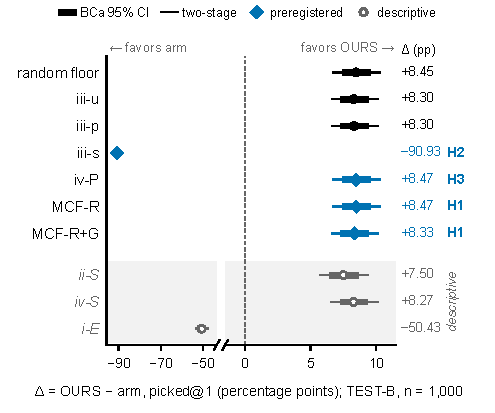
\includegraphics[width=\linewidth]{fig_n3_forest}}{\TODO{figure: forest plot}}
\caption{OURS minus each arm on TEST-B ($n=1{,}000$; percentage points): paired BCa 95\% CI
(thick) and two-stage seed interval (thin); the axis is broken. H1--H3 mark the
preregistered contrasts; ii-S, iv-S and i-E are descriptive. Generated by
\texttt{scripts/fig\_n3\_forest.py} from \texttt{n3\_results.json}.}
\label{fig:forest}
\end{figure}

\begin{sidewaystable}
\caption{TEST-B ($n=$~\nN), primary matcher (\texttt{StructureMatcher} defaults against the
unrelaxed experimental structure); H2 form: EXACT. Information: $L$, true lattice; $c_0$,
true asymmetric-unit centroid; ops, the true space-group operations, enforced; all $c_k$,
the true centroids of all copies. picked@1: seed mean $\pm$ s.d.\ over three seeds (iii-s
is deterministic). $\Delta$: OURS minus arm, paired over crystals, with BCa 95\% CI;
two-stage: the seed-resampling interval. draw@1: a random draw; any@16: any of 16 draws (for
iii-s, its 16 lowest distinct minima).
H1/H2/H3: S, supported; N, not supported (Table~\ref{tab:hyp}); primary family on the OURS
row, the N2 family on the OURS-N2 row. $^{b}$Not computed for iv-P. Per-crystal compute,
evaluation counts and training cost for every arm are in the Supporting Information
(Compute); OURS uses 16 LJ evaluations per crystal.}
\label{tab:main}
\centering
\footnotesize
\setlength{\tabcolsep}{3pt}
\begin{tabular}{llcccccccc}
\toprule
arm & information & repr. & picked@1 (\%) & $\Delta$, pp [95\% CI] & two-stage & draw@1 & any@16 & H1/H2/H3 \\
\midrule
\inputrows{generated/n3_table1.tex}
\bottomrule
\end{tabular}
\end{sidewaystable}

\begin{sidewaystable}
\caption{The preregistered hypotheses on TEST-B: $\Delta$ (pp) of OURS (or OURS-N2) minus the
comparator, BCa 95\% CI, two-stage seed interval, and Holm-adjusted $p$ over the three. For
H1, $\Delta=\min(\Delta_{\text{MCF-R}},\Delta_{\text{MCF-R+G}})$ and both components must
pass. $^{a}$Verdict ``iii-s better''.}
\label{tab:hyp}
\centering
\small
\begin{tabular}{lllcccll}
\toprule
model & & comparator & $\Delta$ & BCa 95\% CI & two-stage & Holm $p$ & verdict \\
\midrule
\inputrows{generated/n3_hyp.tex}
\bottomrule
\end{tabular}
\end{sidewaystable}

\subsection{H1: a learned asymmetric unit against learned independent copies}
MolCrystalFlow, retrained with its released code on our training set and given the true
lattice and the true centroids of all copies, reproduces \nMcfRPick\% of the test
structures (MCF-R) and \nMcfRGPick\% with the symmetry scan (MCF-R+G). OURS exceeds both:
\nHOneRDelta{} pp \nHOneRCI{} against MCF-R and \nHOneGDelta{} pp \nHOneGCI{} against
MCF-R+G, so H1 is supported with $\Delta_{\text{H1}}=$~\nHOneDelta{} pp \nHOneCI{} (Holm
$p=$~\nHOneP). Both two-stage seed intervals exclude zero. H1 measures a bundle: explicit,
enforced symmetry together with our learner, since MCF-R is not given the operations
(although they are recoverable from its inputs; Methods). Before the benchmark, we ran
MolCrystalFlow's released checkpoint on its released test split and scored it with
MolCrystalFlow's own scorer. The five-run median any-of-10 match rates were 29.73\% and
66.53\% at stol 0.9 and 1.0, against the published $\approx$30\% and $\approx$66\%
(Methods; Gate C), satisfying the preregistered check that our harness reproduces the
released checkpoint.
% src: results/n3/gateC.json (5-run medians mcf09 29.733, mcf10 66.533; MCF's scorer); tasks/n3_protocol.md A4 table (lines 1440-1446)

The ablation ii-S separates the two parts. It takes MolCrystalFlow's own sampled
orientations, maps each copy back to an asymmetric-unit orientation, and expands that
exactly, keeping the lowest-energy candidate. Through the identity
$\Delta(\text{OURS}-\text{MCF-R+G})=\Delta(\text{ii-S}-\text{MCF-R+G})+\Delta(\text{OURS}-\text{ii-S})$,
our learner adds \nLearnDelta{} pp \nLearnCI{} over MCF's orientations inside the same exact
expansion (ablation estimate), and the other term is \nExpDelta{} pp \nExpCI. These are
descriptive, with no test. The advantage is not confined to small cells: on the crystals
whose exported MolCrystalFlow cell holds three or more molecules, the smaller of the two H1
differences is \nZmcfMin{} pp.

\subsection{H2: physics-based search}
The classical search iii-s is given exactly what OURS is given and searches over
$R_{\text{asym}}$ with a universal interatomic potential (FF$^\ast$; Methods), keeping the
lowest minimum. It reproduces \nSearchPick\% of the unrelaxed experimental structures, and
OURS minus iii-s is \nHTwoDelta{} pp \nHTwoCI{} (Holm $p=$~\nHTwoP). H2 is not supported.
The comparison was preregistered in its EXACT form, which scores the search's minimised
structure against the unrelaxed experimental one; this form was fixed on the selection set
because the potential holds the experimental orientation there. On TEST-B, when the
experimental structures are minimised over orientation with FF$^\ast$, \nFFAnchN{} converge and
still match under the primary matcher (\nAnchPct\%), \nFFDriftN{} converge but no longer match,
and \nFFUnresN{} do not converge; the shortfall is
the same on the anchored crystals (\nAnchDelta{} pp, \nAnchCI). The potential's training
data (OMC25) overlap with organic molecular crystals; on the \nOmcN{} test crystals whose
CSD refcode family is not in OMC25 the difference is \nOmcDelta{} pp \nOmcCI{} (descriptive).

Minimising OURS's own draws with the same potential (i-E, descriptive) raises its rate to
\nIEPick\%; i-E minus iii-s is still \nIEvsSearchDelta{} pp \nIEvsSearchCI. With the lattice,
operations and position given, only three rotational degrees of freedom remain, a
multi-start search with an accurate potential covers them well, and the learned model does
not compete with it on accuracy. The protocol registered no compute hypothesis, so we make
no claim about speed; it does require per-arm compute to be reported descriptively, and the
Supporting Information (Compute) does so.

\subsection{H3: the previous architecture}
Our previous architecture, retrained on this task with per-copy operation labels, mirrored
conformers and absolute orientation targets (iv-P), reproduced no test structure in any seed
(\nIvPPick\%); OURS exceeds it by \nHThreeDelta{} pp
\nHThreeCI{} (Holm $p=$~\nHThreeP), and H3 is supported. Taking the identity copy's predicted
orientation as $R_{\text{asym}}$ and expanding it exactly (iv-S, descriptive) gives
\nIvSPick\%.

\subsection{Strata and robustness}
Table~\ref{tab:strata} breaks picked@1 down by the number of molecules in the cell, the
exported MolCrystalFlow cell size, space-group class, handedness, formula overlap with
training, and overlap with the potential's training data. These rows are descriptive, with
no tests, and strata smaller than 30 crystals are marked. OURS lies between \nOursStratMin\%
and \nOursStratMax\% on every stratum of at least 30 crystals, and the search between
\nSearchStratMin\% and \nSearchStratMax\%. The second model family, OURS-N2,
reaches \nOursNtwoPick~$\pm$~\nOursNtwoSd\% and gives the same verdicts on H1--H3
(Table~\ref{tab:hyp}). Secondary matchers, ensembles, continuous endpoints, the
diagnostics of MolCrystalFlow's invariances and the DEV-TEST results are in the Supporting
Information.

\begin{sidewaystable}
\caption{Descriptive strata on TEST-B: seed-mean picked@1 (\%) per arm. $K$, molecules in
the cell; $z_\mathrm{MCF}$, molecules in the exported MolCrystalFlow cell; mixed
handedness, cells holding both enantiomorphs of the conformer; formula-disjoint, no formula
shared with training; OMC25 non-overlap, CSD refcode family not in the potential's OMC25
training data; Sohncke, space groups with proper operations only; other, non-centrosymmetric
groups that contain improper operations. The FF$^\ast$
truth label is reported for the H2 pair only. $^{\dagger}$Fewer than 30 crystals; too small
to interpret.}
\label{tab:strata}
\centering
\small
\setlength{\tabcolsep}{3pt}
\begin{tabular}{llrccccccccc}
\toprule
stratum & & $n$ & floor & iii-u & iii-p & iii-s & iv-P & MCF-R & MCF-R+G & OURS & OURS-N2 \\
\midrule
\inputrows{generated/n3_table2.tex}
\bottomrule
\end{tabular}
\end{sidewaystable}

\subsection{Limitations}
The task gives the true lattice, operations and asymmetric-unit centroid, restricts the test
set to $Z'=1$ general-position crystals and holds each conformer rigid at its experimental
geometry, so nothing here measures crystal structure prediction. Even on this reduced task
the learned model's median orientation error is about \nOursGeoMed$^\circ$, and it falls far
short of physics-based search with the same information. MolCrystalFlow ran in our harness
on an exported primitive cell, so H1 compares a bundle of enforced symmetry and learner
rather than learners alone. The interatomic potential's training data overlap with organic
crystals. The diagnostics of MolCrystalFlow's invariances are approximate, and DEV-TEST is not
confirmatory. The protocol's optional second-tier diagnostics, which would have measured
sensitivity to noisy centroids among other things, were not run. The learned arms select
among their unrelaxed candidates with a steric Lennard-Jones energy; we did not test whether
that selection is robust to other potentials such as OPLS, GAFF or UFF.

% =====================================================================
\section{Conclusions}
% =====================================================================
In a preregistered benchmark of molecular-crystal orientation completion, predicting the
asymmetric-unit orientation and building the crystal by exact space-group expansion
outperformed a learned model of independent copies given the true lattice and the true
centroids of all copies (H1) and our previous architecture (H3). As an ablation estimate,
our learner adds \nLearnDelta{} pp \nLearnCI{} over MolCrystalFlow's orientations inside the
same exact expansion. A physics-based search given the same information was far more accurate
(H2 not supported). For learned molecular-crystal models, the results favour predicting
the asymmetric unit and expanding it exactly over predicting every copy; whether that
holds once the lattice and position must also be generated is not tested here.

\IfFileExists{sections/methods.tex}{% =====================================================================
% methods.tex -- Methods for the N3 resubmission (ACS Omega places Methods
% after Conclusions). Procedures only; no N3 result numbers.
% P = tasks/n3_protocol.md (frozen v3 with amendments A1-A4 and the step-5b
% clarifications). Citation placeholders use \CITEME{...}, which main.tex
% already defines. Uses \ref{tab:repr} (Table R, defined in main.tex) and
% defines \label{tab:info} (Table 0) and \label{eq:expand}. Cross-references to the Supporting Information are by name (amendment,
% disclosure letter), because the SI is a separate document.
% =====================================================================
\section{Methods}

\subsection{Task and inputs}

The benchmark asks for orientation completion of $Z'=1$ molecular crystals whose
molecule sits on a general position. OURS and the classical arms were given the
experimental lattice $L$ (cell vectors as rows); the $K$ space-group operations $(W_k,t_k)$ in
the crystal's own CSD setting, from pymatgen's SpacegroupAnalyzer (symprec
0.1)\cite{ong2013pymatgen,togo2024spglib} run on the experimental structure; the
fractional centroid $c_0$ of the asymmetric-unit molecule; and its rigid
experimental conformer as centered coordinates $l_a$ in a body frame fixed by the conformer
alone (the principal axes of its gyration tensor, ordered by spread, with signs set by an
element-weighted third moment and a right-handed frame), so the true $R_{\mathrm{asym}}$ is the
rotation from that body frame into the crystal's Cartesian frame. Each of these arms predicted one rotation,
the asymmetric-unit orientation $R_{\mathrm{asym}}\in\mathrm{SO}(3)$, and exact
space-group expansion placed atom $a$ of copy $k$ at
\begin{equation}
x_{k,a}=L^{\top}c_k+C_kR_{\mathrm{asym}}l_a,\qquad
c_k=W_kc_0+t_k\ (\mathrm{mod}\ 1),\qquad
C_k=L^{\top}W_kL^{-\top}.
\label{eq:expand}
\end{equation}
Because $\det C_k=\pm1$, improper operations produce the mirror-image copies
directly, and the operations fix $Z=K$, $Z'=1$ and the handedness of every copy.
The reference structure for every arm was the parsed experimental crystal.
A random-orientation floor was preregistered as the check that the task is not
trivial.
Table~\ref{tab:info} lists the information each arm received.
% src: tasks/n3_protocol.md:26-36,135; scripts/g2_asym_baselines.py:36-50,74-89

% (Table 0, \label{tab:info}, moved into Results: Benchmark design)


\subsection{Data and splits}

All crystals came from one seeded random sample of the Cambridge Structural
Database (CSD)\cite{groom2016csd}, exported with the CSD Python API (organic, not
organometallic, no disorder, three-dimensional coordinates, not polymeric,
$R\le7.5\%$, $Z'\le2$, at most 64 atoms in the largest component) and parsed into
rigid molecules with mirror-image copies allowed. A crystal was eligible when its
molecules had equal atom counts and numbered $K$. The first 3,500 refcodes (2,852
parsed, 1,987 eligible) were split with seed 0 into DEV-TEST (200), VAL (100) and
TRAIN (1,687). DEV-TEST was scored while OURS was developed and is reported only as
a secondary set (Supporting Information, Disclosures).
% src: scripts/csd_export.py:9-22,62-64; data/csd_mol_scale_big/manifest.csv (maxima: R 7.5, Z' 2.0, 64 atoms); tasks/n3_protocol.md:70-71,92,164-198,895; scripts/g2_asym_baselines.py:53-71

TEST-B (confirmatory) and SEL (selection supplement) came from the next 4,500
refcodes of the same stream; no development step of this benchmark parsed or scored them,
although the legacy pipeline of the earlier version had parsed this pool and trained on it
(no legacy checkpoint is used; Supporting Information, Disclosures). They
were built by input-side steps only: the rigid-molecule parse and its rebuild check
(3,632 kept); an expansion check requiring that the orbit points $W_kc_0+t_k$ match
the stored centroids one to one and that expanding the true orientation reproduce
the experimental structure under StructureMatcher (1,157 removed, nearly all not
$Z'=1$ general position); removal of crystals sharing a six-letter refcode family
with the development corpus or a molecular Weisfeiler--Lehman graph
hash\cite{shervashidze2011wl} (computed with NetworkX\cite{hagberg2008networkx}) with its
1,987 molecules (22
removed); and, after a seeded permutation (seed 20261001), one crystal per refcode
family (2,448 kept). SEL is the first 300 and TEST-B the next 1,000 (679
centrosymmetric, 270 Sohncke and 51 other crystals). Both refcode lists were
committed with SHA-256 hashes before any arm produced output on them, and they,
not a re-run of the order-dependent parse, define the sets. VALSEL (VAL then SEL,
400 crystals) served for every choice.
% src: tasks/n3_protocol.md:72-79,80-126,1098-1110; results/n3/n3_build_testB.json

The CSD is license-restricted. Only refcodes, code and JSON summaries were
committed; no coordinates, exported files, trained checkpoints or arm outputs
were redistributed, and a licensed CSD installation reproduces every set from the
refcode lists. No arm trained on anything but TRAIN, and MCF's released
checkpoints were used only in a harness check.
% src: tasks/n3_protocol.md:137-141,1066-1068; paper/submissions/ACSOmega/main.tex:571-578; .gitignore:10

\subsection{Model}

OURS is a flow-matching model\cite{lipman2023flowmatching,chen2024riemannian} on
$\mathrm{SO}(3)$ for $R_{\mathrm{asym}}$ alone, with a learned pairwise torque as
its velocity field. For a trial orientation $R$, each atom $i$ of the
asymmetric-unit molecule was paired with each atom $j$ of the copies and periodic
images that eq~\ref{eq:expand} places within an 8~\AA\ cutoff. A
multilayer perceptron (two hidden layers of 64 units) mapped 16 radial basis
functions of the distance $d_{ij}$, learned element embeddings of both atoms and
Fourier features of the flow time $t$ to a scalar $s_{ij}$, damped smoothly to zero
at 8~\AA, and
\begin{equation}
f_i=\sum_j s_{ij}\,\frac{x_i-x_j}{d_{ij}},\qquad
\omega=\sum_i (x_i-L^{\top}c_0)\times f_i
\end{equation}
was read as the angular velocity of the asymmetric unit. Built from interatomic
vectors only, the field rotates with the crystal, and the symmetry copies, mirror
images included, enter only through exact expansion. The network has 9,473
parameters.
% src: scripts/g2_learned_flow.py:1-14,44-66,69-127; results/vast_g2/eval_s0.pt (parameter count)

Training used conditional flow matching on $\mathrm{SO}(3)$. With $R_0$
Haar-random, $t$ uniform on $[0,0.98)$ and $R_1$ the experimental orientation, the
loss was $\lVert\omega_\theta(R_t,t)-u\rVert^2$ at the geodesic point
$R_t=\exp(t\log(R_1R_0^{\top}))R_0$, with target $u=\log(R_1R_t^{\top})/(1-t)$.
Each AdamW step (learning rate $10^{-3}$, weight decay $10^{-4}$) used one crystal
and one draw. Seeds 0, 1 and 2 were trained on CPU. The runs were scheduled for 40
epochs but stopped after nine, and the checkpoints used here were saved after epoch 8
(Supporting Information). For each seed, the epoch with the lowest validation loss among
those eight was kept (epochs 1, 8 and 4). These checkpoints predate the benchmark, and
they were kept after DEV-TEST had been seen (Supporting Information, Disclosures).
Sampling took 40 Euler steps on $\mathrm{SO}(3)$ from 16 Haar-random starts per crystal,
and the selector, chosen on VAL during development, returned the draw with the lowest
unrelaxed steric energy. Per-crystal seeds were $80000+i$ on TEST-B and $90000+i$ on SEL
($i$, the position in the frozen list); VAL and DEV-TEST reused the draws stored during
development, re-matched from their rotations. OURS-N2, a sensitivity variant, is the same
network retrained for 30 epochs with eight draws per
crystal per step, cosine learning-rate decay and fixed validation draws, its
checkpoints chosen on VAL.
% src: scripts/g2_learned_flow.py:130-144,155 (--epochs default 40),184-227; results/vast_g2/eval_s{0,1,2}.pt (hist: epochs 0-7; best 0/7/3, zero-based; epoch 7 = the per-epoch resume checkpoint after the eighth epoch); results/vast_g2/g2_learned_s{0,1,2}.log and .resume.pt (records end at epoch index 8, no final checkpoint written); scripts/n3_ours.py:93 (loads best_state); scripts/g2_rank.py:44-51; tasks/n3_protocol.md:19-20,156-162,242-244,274-275,362-368; scripts/g2_train_v2.py:1-12; tasks/omega_rebuild_plan.md:67-68,120-141

\subsection{Comparators}

MolCrystalFlow\cite{zeng2026molcrystalflow} (MCF) generates a lattice, centroids
and one orientation per copy, each copy carrying its own conformer and a handedness
flag $\chi$. We ran its released code (commit 3c493f8) in a fork limited to six
patches, listed with their diff in the Supporting Information: added atom types, a bug
fix, a clamp that holds the lattice and centroids at their inputs, a device fix, a seeding
fix, and a pair of verified speed-ups. Crystals were exported through MCF's own
preprocessing and feature code, with centered cells reduced to their primitive cells. An
export check verified atom-by-atom round trips and matches to the truth on every set.
Before any MCF training, a harness check verified that our harness reproduces MCF's
published results with its released Thurlemann
checkpoint\cite{zeng2026molcrystalflowdata,thurlemann2023regularized} (within $\pm5$
percentage points of its Fig.~3a at stol 0.9 and 1.0), that the patches leave the
computation unchanged, and that the clamp is exact; it passed after corrections recorded
as a protocol amendment (Supporting Information, Amendments).
% src: tasks/n3_protocol.md:372-393,402-433,438-505,1431-1506; results/n3/n3_selection.json:"gate_c"

MCF-R held the lattice and all $z_{\mathrm{MCF}}$ centroids at the truth in
training and sampling, so only orientations were learned and generated. It used
MCF's released configuration with the translation and lattice noise and their loss terms disabled,
three seeds, 1,715 epochs (24,010 optimizer steps, close to the 23,700 of MCF's
own run) and 16 samples per crystal with 50 Euler steps. Because MCF's network sees
orientations only through relative rotations, its sampled orientations are
invariant, up to a branch-cut effect (Supporting Information), under a group $H$ of common
rotations set by $z_{\mathrm{MCF}}$ ($\mathrm{SO}(3)$ for $z_{\mathrm{MCF}}=1$,
O(2) for 2, D$_2$ for 3 or more). MCF-R+G therefore scanned $H$ for each draw
(both cosets on a 2$^\circ$ grid, or the four D$_2$ elements) and kept the member
with the lowest steric energy; it uses no truth. For $z_{\mathrm{MCF}}=1$ no scan is run,
so MCF-R+G equals MCF-R there. The network is equivariant away from the branch cut, but the
sampler's invariance is only approximate: after 50 steps, the largest element-wise
difference between the rotation matrices sampled from a prior draw and from its rotated
copy is of order one (Supporting Information, diagnostic (a)). MCF-A trained MCF's released joint objective (lattice, centroids and
orientations generated). It receives less information than OURS, is reported in a
separate context table and enters no hypothesis.
% src: tasks/n3_protocol.md:507-531,556-584,598-613

The classical arms received the inputs of OURS and moved only
$R_{\mathrm{asym}}$. iii-u drew 16 Haar-random rotations per crystal under three
seed bases; with the RANDOM selector these draws are the random floor. iii-p
applied the development steric press (80 Adam steps on the orientation) to them.
iii-s, the physics search, expanded the 4,608 orientations of an incremental Hopf
grid (about 15$^\circ$ apart)\cite{yershova2010hopf,gorski2005healpix}, kept the 64 with
the lowest unrelaxed steric energy, and minimized each over orientation with the
machine-learned potential UMA s-1p1 (OMC task)\cite{wood2025uma,fairchem2026core}, which
the MCF authors use for their own rigid-body relaxation\cite{zeng2026molcrystalflow}
(denoted FF*). Minimization used
L-BFGS\cite{liu1989lbfgs}
(at most 100 energy-and-gradient evaluations; converged when the orientation
gradient per molecule fell below 0.01~eV\,rad$^{-1}$), minima within 2$^\circ$
were merged, and the lowest-energy minimum was the pick. FF* ran in float32 with
the same settings in every job. For FF* evaluations the X--H bonds were set to the
CSD neutron-normalized lengths (C--H 1.089, N--H 1.015, O--H
0.993~\AA)\cite{allen2010xh}; the returned orientation was
applied to the original conformer, so every scored structure keeps the
experimental hydrogen positions. Because UMA's organic-crystal training data, OMC25, derive from
CSD molecules\cite{gharakhanyan2026omc25,stuke2020oe62}, H2 is also reported on the TEST-B crystals whose
refcode family is absent from it.
% src: tasks/n3_protocol.md:656-726,1378-1386

iv-P ran our previous architecture, SymMC-Flow\cite{cai2026symmcflow}, with its
published defaults (an E(n)-equivariant conformer encoder\cite{satorras2021egnn}
and pair-bias attention across molecules) on per-copy items built from the
asymmetric unit: true centroids for all $K$ copies, a mirrored conformer for
improper copies, and a coset label (space group, $W_k$) from a table built on
TRAIN. Only the orientation loss was used (lattice and centroid weights 0, a
disclosed deviation), for 60 epochs, with seed 0 at three learning rates and seeds
1 and 2 at the chosen one. Sampling integrated the orientation flow with RK4 (50
steps) from $K$ independent Haar priors, without symmetrization.
% src: tasks/n3_protocol.md:762-805; symmc_flow/config.py:6-37

Three descriptive ablations were run. ii-S placed MCF's orientations inside our exact
expansion: each MCF-R+G copy was pulled back to an asymmetric-unit estimate by
Kabsch alignment\cite{kabsch1976solution,kabsch1978discussion}, each estimate was expanded, and the
lowest-energy expansion was kept. iv-S expanded iv-P's identity-copy orientation.
i-E minimized all 16 OURS draws under FF* and picked the lowest FF* energy, which
separates the learned proposal from the energy model.
% src: tasks/n3_protocol.md:586-596,750-754,806-808

\subsection{Selection and matching}

The primary matcher was pymatgen's StructureMatcher\cite{ong2013pymatgen} with
default settings (ltol 0.2, stol 0.3, angle\_tol 5$^\circ$), computed as
fit(truth, candidate) on the unrelaxed experimental structure and the candidate as
emitted. Secondary matchers applied MCF's rule\cite{zeng2026molcrystalflow} (ltol 0.3,
angle\_tol 10$^\circ$, no scaling, a match whenever an RMS distance is returned) at stol 0.5
and 0.8; tolerances this loose are common in generative CSP benchmarks and exceed
pymatgen's defaults\cite{martirossyan2025matching}. One script scored every arm, and no output
was matched against the truth before the scoring step. The denominator was always
the full set: an arm failure counted as a miss, harness crashes were re-run, and
no crystal was dropped or timed out.
% src: tasks/n3_protocol.md:143-162,203-217

Each sampling arm drew 16 samples per crystal and seed (iii-s instead keeps its 16 lowest
distinct minima from a screened, multi-start search), and a selector made one
pick: RANDOM (scored as the exact fraction of matching draws), LJ (lowest steric
energy, a Lennard-Jones sum over intermolecular atom pairs within 6~\AA\ with
contact distances 0.90 times the sum of the van der Waals radii), RESID (learned
arms; lowest residual of one extra forward pass at $t=0.975$) or MODE@$r$ (most
frequent endpoint within a radius $r$ of 0.25 to 1.5~\AA). OURS kept its
development selector and iii-s its physics selector. Every other arm chose its
selector on its own VALSEL draws by seed-summed primary-matcher hits (MCF-A by
picked@1 under MCF's rule at stol 1.0), with ties going to LJ, RESID, MODE@$r$ and
RANDOM in that order. The MCF arms also chose rotation-schedule rates (MCF-R and
MCF-R+G: $s_{uR}\in\{1,2,3,5,10\}$) and one checkpoint per seed, and iv-P its
learning rate and checkpoints. The frozen choices were LJ for every arm except
iii-p (MODE@1.0) and iii-s; $s_{uR}=5$ for MCF-R and MCF-R+G; schedule rates
$(s_{uF},s_{uR})=(9,3)$ for MCF-A; and learning rate $10^{-4}$ for iv-P. The
checkpoints are listed in the Supporting Information.
% src: tasks/n3_protocol.md:251-276,545-554,576-582,605-609,792-802; symmc_flow/rigid_press.py:30-36,109-146; results/n3/n3_selection.json:236-470

\subsection{Statistics and hypotheses}

The headline estimand was seed-mean picked@1, the outcome of the single pick per
crystal averaged over three seeds (one run for iii-s); draw@1, any@16 and
48-draw ensembles were descriptive. For crystal $i$ and comparator $A$,
$d_i=h_i^{\mathrm{OURS}}-h_i^{A}$, with $h_i$ the seed-mean outcome, and $\Delta$
is the mean of $d_i$. Contrasts used a two-sided paired sign-flip test on
$\sum_i d_i$, computed exactly: because every $d_i$ is a multiple of $1/48$ (seed means
are multiples of $1/3$, random-selector expectations of $1/16$), the null distribution of
the sum is the convolution of the individual sign-flip distributions on that grid. The
preregistered hypotheses, one family tested on
TEST-B with Holm's step-down procedure\cite{holm1979simple} at family-wise
$\alpha=0.05$, were: H1, OURS against MCF-R and against MCF-R+G as an
intersection-union test ($p=\max(p_R,p_G)$, $\Delta_{\mathrm{H1}}=\min(\Delta_R,
\Delta_G)$, supported only if both differences are positive); H2, OURS against
iii-s; and H3, OURS against iv-P. A verdict names a better arm only at adjusted
$p<0.05$; otherwise the difference is reported as not resolved. $\Delta$ is
given in percentage points with a paired crystal-bootstrap BCa 95\%
interval\cite{efron1987better} (10,000 resamples). A two-stage
bootstrap over seeds and then crystals (10,000 replicates) measured training-seed
sensitivity; a supported hypothesis whose interval contains zero is worded ``not
shown to exceed seed-to-seed training variation''. H1--H3 were repeated with
OURS-N2 as a separate family. Secondary matchers, MCF-A, ablations, DEV-TEST and
strata ($K$, $z_{\mathrm{MCF}}$, centrosymmetric, Sohncke or other, mixed
handedness, formula absent from TRAIN, OMC25 non-overlap) carry 95\% intervals
only.
% src: tasks/n3_protocol.md:219-233,278-316,336-357,818-822

The H2 form was fixed on VALSEL before any candidate was minimized. The 400 VALSEL
truths were minimized under FF*; if at least 50\% converged and still matched the
experimental structure, H2 would compare unrelaxed outputs (EXACT), and otherwise it
would compare minimized picks with the minimized truth (BASIN). The form was EXACT,
recorded in a public commit before any benchmark candidate was minimized (Supporting
Information), so H2 compares the unrelaxed OURS pick and iii-s's lowest minimum, each with
the unrelaxed experimental structure. Because an EXACT-form difference can come from
crystals whose experimental pose drifts under FF*, every TEST-B truth was also labeled
ANCHORED, DRIFTED or UNRESOLVED, and ``better than physics-based search'' was
reserved for an ANCHORED-subset interval entirely above zero. This and every other
outcome-to-wording rule, including how the ii-S ablation splits the H1 difference,
were fixed before any arm ran.
% src: tasks/n3_protocol.md:727-749,840-873; results/n3/n3_selection.json:121-124; git 1aff111

\subsection{Representability}

Table~\ref{tab:repr} counts the TEST-B and DEV-TEST crystals whose
experimental structure each
representation can emit, computed before any sampling and under every matcher: (a)
exact expansion, as used by OURS and the classical arms (all of TEST-B by
construction); (b) MCF's per-copy representation; (c) the information of MCF's
released structure-prediction driver, one conformer and one $\chi$ for all copies,
as the lowest-RMSD homochiral approximant found (each improper copy replaced by the
lowest-RMSD proper rotation onto its mirror found by a multi-start search); and (d) the
legacy det+1 parser of our previous work, which accepts proper rotations only. No
representability claim is made relative to MCF's per-copy representation.
% src: tasks/n3_protocol.md:876-909

\subsection{Preregistration and execution}

The protocol was committed and pushed to the public repository\cite{cai2026symmcflow}
on September 28, 2026, before any comparator was trained and before any arm was sampled or
scored under it. The OURS and OURS-N2 checkpoints, and OURS's development results on VAL and
DEV-TEST, already existed (Supporting Information, Disclosures).
Later changes were made only through dated amendments and clarifications, each recording
which outputs existed when it was made, and every one preceded the first scoring of TEST-B;
the Supporting Information lists every record with its date and commit. All selection choices, the H2 form and the list of permitted TEST-B and DEV-TEST
runs with their seeds were committed and pushed before any TEST-B or DEV-TEST input reached
the compute cluster. Exactly the listed runs were made, their outputs were retrieved with
checksums, the CSD-derived files on the cluster were deleted, and both sets were scored
once. The results were committed and pushed before they were interpreted. Training of
the comparators (MCF and iv-P), sampling and FF* jobs ran on NVIDIA A100 nodes of the
Purdue Anvil cluster\cite{song2022anvil} in one container image, and
scoring used the cluster's CPU cores; the OURS and OURS-N2 checkpoints had been trained on
CPU before the benchmark.
% src: tasks/n3_protocol.md:1-17,967-1015,1367-1377; results/n3/n3_selection.json:1-4; tasks/n3_step9_clarification_2026-11-15.md:11-27; tasks/n3_step4_record_2026-10-11.md:878-944,1043-1045; git log 8f7e494, 772a36e, f1c713a
}{\section{Methods}\TODO{sections/methods.tex}}

\begin{acknowledgement}
The author thanks the Cambridge Crystallographic Data Centre for access to the Cambridge
Structural Database under an academic licence. This work used Anvil at Purdue University
through allocation CHE260157 from the Advanced Cyberinfrastructure Coordination Ecosystem:
Services \& Support (ACCESS) program, which is supported by U.S. National Science
Foundation grants \#2138259, \#2138286, \#2138307, \#2137603 and \#2138296
\TODO{confirm the allocation wording, add the Anvil citation, and list any other compute
used for N3}. The author declares no competing financial interest. During this work the
author used Claude (Anthropic) as a coding and writing assistant: it implemented analysis
and benchmark code under the author's direction and drafted text that the author revised;
the author reviewed all output and takes full responsibility for the content
\TODO{Frank: confirm the AI-use wording}.
\end{acknowledgement}

\section*{Data and Software Availability}
The source code, the preregistered protocol and its amendments, the frozen model selection,
the refcode lists that define every set, and the numeric results (\texttt{n3\_results.json})
are openly available at \url{https://github.com/fronkt/symmc-flow} and archived at
Zenodo\cite{cai2026symmcflow} \TODO{mint a new Zenodo version and cite the results
commit}. The Cambridge Structural Database is licence-restricted; the crystal structures are
not redistributed, and the refcode lists reproduce every set from a licensed CSD
installation.

\begin{suppinfo}
Preregistration, amendments and disclosures, with the checkpoints of every arm; secondary
matchers and the Haar floor; ensembles, any@48 and continuous endpoints; ablations and
descriptive arms (ii-S, iv-S, i-E, steric basin); the MolCrystalFlow fork, its diagnostics and
the context arms; strata and representability in full; DEV-TEST results (not confirmatory);
the VALSEL selection grids; run health and gates; compute; the training and test sets
(Figure S2); representative successes and failures (Figure S3) (PDF).
\end{suppinfo}

\bibliography{references}

\end{document}
